\section{Anexos}

\subsection{Registro fotográfico de capacitaciones presenciales}

\begin{indentedsubsection}
A continuación se presentan las evidencias fotográficas de las sesiones de capacitación presencial llevadas a cabo con el personal operativo y la gerencia de Machu Picchu Exclusive Tours E.I.R.L. Estas sesiones se enfocaron en la adopción del sistema Odoo para la gestión del CRM turístico, el control de reservas e itinerarios y el seguimiento de actividades.

\begin{figure}[h]
    \centering
    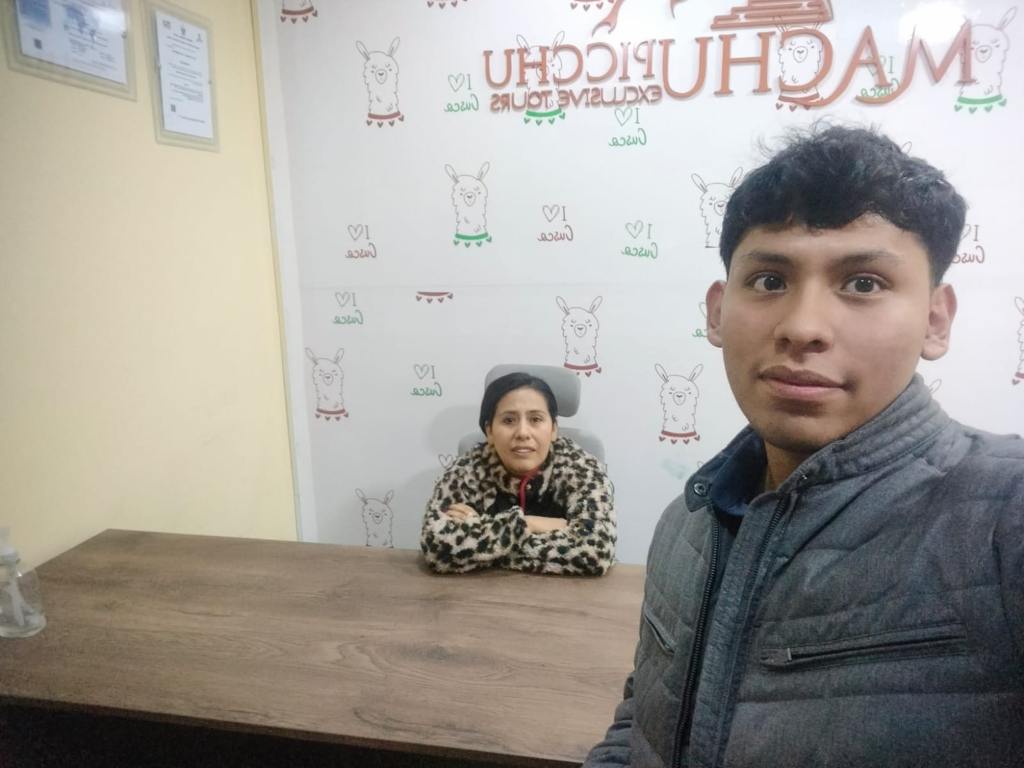
\includegraphics[width=0.8\textwidth]{assets/capacitacion-presencial-1.png}
    \caption{Sesión práctica presencial y coordinación operativa de la implementación}
\end{figure}

\begin{figure}[h]
    \centering
    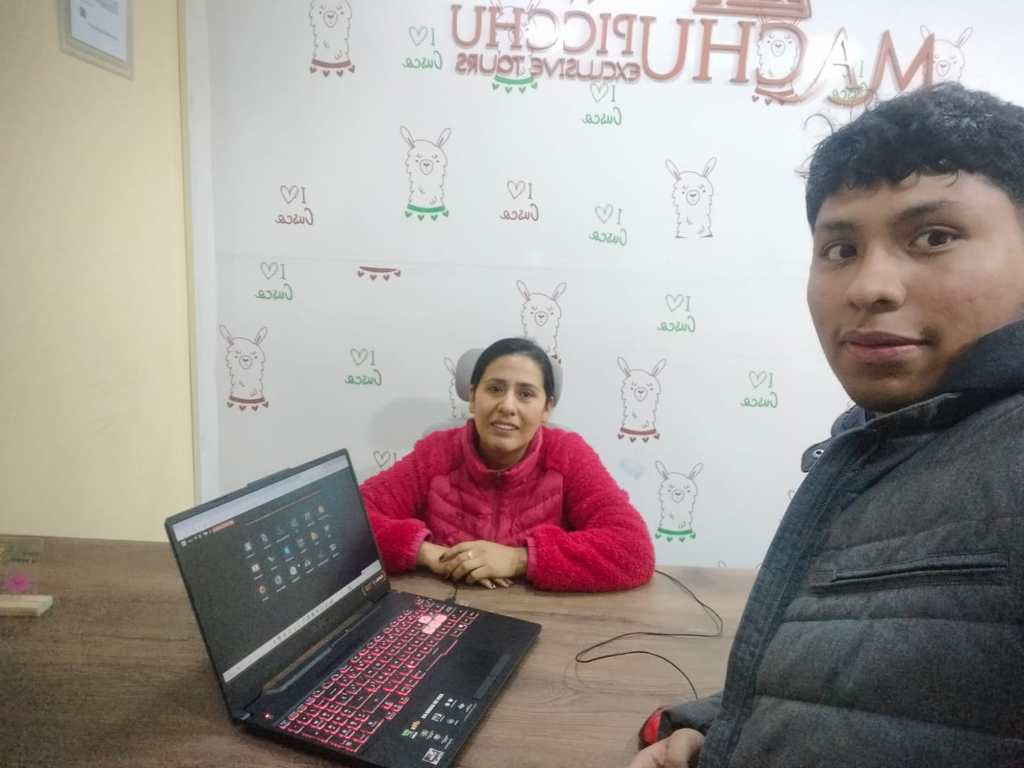
\includegraphics[width=0.8\textwidth]{assets/capacitacion-presencial-2.png}
    \caption{Capacitación interactiva en la interfaz de Odoo para el control de reservas}
\end{figure}

\end{indentedsubsection}

\subsection{Registro de capacitación virtual}

\begin{indentedsubsection}
Adicionalmente, se realizaron sesiones de capacitación virtual y asistencia remota para reforzar el uso del sistema y guiar a los usuarios en la navegación por los diferentes módulos del sistema Odoo (CRM, Contactos, Ventas, Proyectos).

\begin{figure}[h]
    \centering
    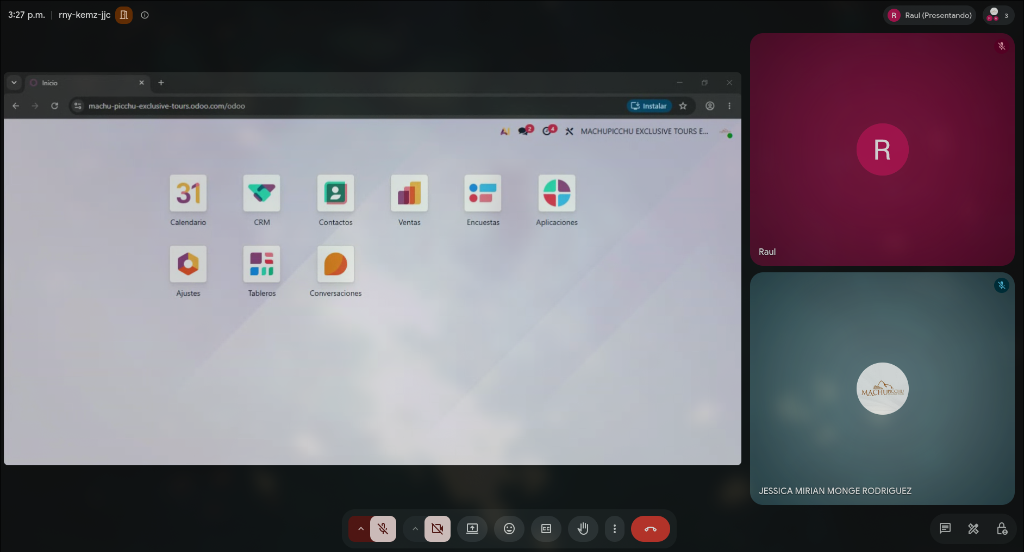
\includegraphics[width=0.8\textwidth]{assets/capacitacion-virtual-1.png}
    \caption{Sesión de capacitación virtual remota sobre el entorno Odoo de la empresa}
\end{figure}

\begin{figure}[h]
    \centering
    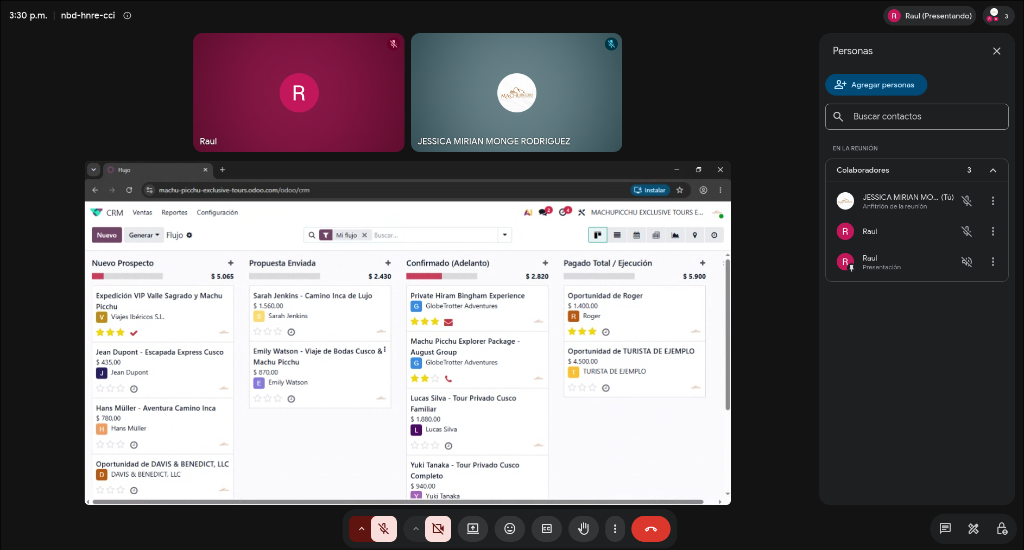
\includegraphics[width=0.8\textwidth]{assets/capacitacion-virtual-2.png}
    \caption{Taller virtual práctico sobre el control de flujos de CRM y pipeline turístico}
\end{figure}

\end{indentedsubsection}
